% Volume III chapter: The classical sources (von Mangoldt, Ramanujan, Hardy and Littlewood, Hardy Littlewood Polya, Montgomery and Vaughan). Sources: misc/reviews/nick-ch17-classics/chapter17/chH_classics.tex lines 1 to 207; referee report CL17 (M1 to M13 and minors); verification CL17. 17 Nov 2026.
% Coordinator notes: uses the environment computation and the label prefixes bo:, cl:; cites yo:prop:tent, yo:thm:D, ch:riesz; figure fig/v3/cl_ramanujan.pdf (the plotted range and correlation were confirmed, only three printed point values were wrong); new bibliography in ch/nc_v3_classics_bib.tex (Lehmer88 is also in misc/vol3/bib_new.tex).
\label{ch:classics}

The oscillator of Chapter~\ref{bo:ch:bondesson} was found by following Bondesson's letter and the Thorin measure. Once found, it turns out to have ancestors. This chapter reads four of them: von Mangoldt's proof of Riemann's formula (1895), Ramanujan's paper on highly composite numbers (1915), the long Acta paper of Hardy and Littlewood (1916) with the criterion of Riesz, and the book \emph{Inequalities} of Hardy, Littlewood and P\'olya (1934). Each is read for what it says about the oscillator, and each reading is checked by a computation. The chapter is from an unrefereed note of Polson (November 2026).

The oscillator is $f(L)=\sum_{\gamma>0}2(1-\cos\gamma L)/\gamma^2$ under RH, with values in $[0,W]$, $W=4\sum_{\gamma>0}\gamma^{-2}=0.09242$ (Theorem~\ref{bo:thm:osc}); it is half the function $D$ of Proposition~\ref{yo:prop:tent}. Ramanujan, assuming RH, bounded a different sum, $\sum_\rho x^\rho/\rho^2$, symmetrically by $\sqrt x\sum_\rho|\rho|^{-2}=(2+\gamma_E-\log4\pi)\sqrt x$, a band of total width $0.09238$. The two widths differ by $3.7\times10^{-5}$. After a shift by $W/2$ the normalised sum and the oscillator differ by a series of size at most $0.0015$, and by at most $0.0012$ on the computed range, and computed from the primes to $10^9$ they move together with correlation $0.998$. Ramanujan did not have the one sided band $[0,W]$ and stated no converse. The converse is the argument of Landau, as in Ingham \cite{Ingham32} and in Theorem~\ref{yo:thm:D} of Volume II. The other readings explain why the oscillator works where older criteria are numerically blind, and supply the inequality that gives finite range versions of its mean values.

\section{Von Mangoldt, 1895: the formula that is integrated}\label{cl:sec:vm}

Riemann stated his formula for the prime counting function in 1859 without a complete proof. Von Mangoldt gave the first proof in \emph{Zu Riemanns Abhandlung}, Journal f\"ur die reine und angewandte Mathematik 114 (1895), 255 to 305 \cite{vonMangoldt95}, by way of the function $\psi(x)=\sum_{n\le x}\Lambda(n)$ that now carries his name in $\Lambda$. His formula is
\[
\psi_0(x)=x-\sum_\rho\frac{x^\rho}{\rho}-\log2\pi-\frac12\log\bigl(1-x^{-2}\bigr)\qquad(x>1),
\]
with $\psi_0$ the average of the left and right limits and the sum over zeros taken symmetrically. Every term of it reappears in the oscillator. The $x$ is the pole, $e^{L/2}$ in Theorem~\ref{bo:thm:osc}; the logarithm is the trivial zeros, the sum $\sum_ke^{-(2k+\frac12)L}/(2k)$; the constant $\log2\pi=\zeta'(0)/\zeta(0)$ is fixed by the value at the origin; and the sum over zeros becomes $\sum_\rho e^{(\rho-\frac12)L}/\rho$ after multiplying by $x^{-1/2}$, with $L=\log x$. In this form von Mangoldt's formula is, up to explicit terms and a running average of the same error (Proposition~\ref{bo:prop:velocity}), the derivative $f'(L)$ of the oscillator, whose zero terms are of size $\gamma^{-1}$. The oscillator, with terms of size $\gamma^{-2}$, is one integration of it in $L$.

What integration buys is convergence. Von Mangoldt's sum converges only conditionally, with terms of size $x^{1/2}/\gamma$, and truncating it at height $T$ leaves an error of order $x\log^2(xT)/T$. Integrated once in $\log x$ the terms become $x^\rho/\rho^2$, which converge absolutely and, after the factor $x^{-1/2}$, uniformly in $L$, and under RH the error of truncation is at most $\sqrt x\sum_{\gamma>T}2\gamma^{-2}$. The sign of the oscillator does not come from the integration. It comes from the centring at $\rho=\frac12$, as explained after Theorem~\ref{cl:thm:band}.

\begin{computation}\label{cl:comp:vm}
Truncation at height $T$ (computed, with $\psi$ from the primes at the exact value of $x$, and $T$ meaning the zeros with $|\gamma|<T$; for $T=7000$ these are the first $6703$ zeros). The second column is $|\psi_0(x)-(x-\sum_{|\gamma|<T}x^\rho/\rho-\log2\pi-\frac12\log(1-x^{-2}))|/\sqrt x$. The third is the same quantity for the integrated sum $\sum_\rho x^\rho/\rho^2$, with the full sum taken from the primes by Proposition~\ref{cl:prop:ramform}.
\begin{center}\small
\begin{tabular}{@{}lccc@{}}
\toprule
$x$ & $T$ & von Mangoldt & integrated once\\
\midrule
$10^3$ & $100$ & $8.2\times10^{-2}$ & $7.5\times10^{-4}$\\
$10^3$ & $7000$ & $1.6\times10^{-3}$ & $6.6\times10^{-7}$\\
$10^5$ & $100$ & $6.7\times10^{-2}$ & $2.1\times10^{-4}$\\
$10^5$ & $7000$ & $8.6\times10^{-3}$ & $1.5\times10^{-7}$\\
$10^7$ & $100$ & $2.2\times10^{-1}$ & $1.1\times10^{-4}$\\
$10^7$ & $7000$ & $5.0\times10^{-3}$ & $1.4\times10^{-6}$\\
\bottomrule
\end{tabular}
\end{center}
The entries at $T=7000$ depend on the phase of the neglected zeros and on the exact cutoff, so they are good to the order of magnitude only. The point $x=10^3$ lies $3$ units from the prime $997$, inside the zone of Gibbs oscillation at $T=100$.
\end{computation}

At $T=7000$ one integration gains a factor between about two thousand and sixty thousand.

\section{Ramanujan, 1915: the band}\label{cl:sec:ramanujan}

Ramanujan's \emph{Highly composite numbers} appeared in the Proceedings of the London Mathematical Society in 1915 \cite{Ramanujan15}, shortened for reasons of cost. The omitted part, which assumes RH, was published in 1997 with notes by Nicolas and Robin \cite{Ramanujan97}. % UNCHECKED: the equation numbers of the 1997 text were not available; the quoted inequality below was not checked against it (CL17 M3)
In it Ramanujan, as we read the annotated edition, writes $\vartheta(x)=\sum_{p\le x}\log p$ as $x-\sqrt x-\sum_\rho x^\rho/\rho+O(x^{1/3})$, introduces the remainder
\[
R(x)=\frac{2\sqrt x+\sum_\rho x^\rho/\rho^2}{\log^2x}
\]
in his expansion of $\pi(x)$ in terms of $\operatorname{Li}(\vartheta(x))$, and uses the Hadamard product to get $\sum_\rho1/\rho=1+\frac12(\gamma_E-\log4\pi)$. Here $\gamma_E$ is Euler's constant. Under RH, $|\rho|^2=\rho(1-\rho)$ and $\sum_\rho1/|\rho|^2=2\operatorname{Re}\sum_\rho1/\rho=2+\gamma_E-\log4\pi$, so $|\sum_\rho x^\rho/\rho^2|\le(2+\gamma_E-\log4\pi)\sqrt x$, and he states
\[
(\log4\pi-\gamma_E)\sqrt x\ \le\ R(x)\log^2x\ \le\ (4+\gamma_E-\log4\pi)\sqrt x .
\]
The interval has width $2(2+\gamma_E-\log4\pi)\sqrt x=0.09238\sqrt x$.

This band is close to that of the oscillator, but it is centred differently. Ramanujan's normalised sum is
\[
g(L)=e^{-L/2}\sum_\rho\frac{x^\rho}{\rho^2}=\sum_{\gamma>0}2\operatorname{Re}\frac{e^{i\gamma L}}{(\frac12+i\gamma)^2},
\]
with values in $[-0.04619,0.04619]$. Since $(\frac12+i\gamma)^{-2}=-\gamma^{-2}+O(\gamma^{-3})$, $g=f-\frac W2+O\bigl(\sum\gamma^{-3}\bigr)$: up to a shift by half the width, Ramanujan's sum and the oscillator differ by a uniformly convergent series of size about $10^{-3}$. The two bands differ in width by $4\sum_{\gamma>0}\bigl(\gamma^{-2}-(\frac14+\gamma^2)^{-1}\bigr)=\sum_{\gamma>0}\frac1{\gamma^2(\frac14+\gamma^2)}$, which is $3.7\times10^{-5}$.

\begin{proposition}[Ramanujan's sum from the primes]\label{cl:prop:ramform}
Unconditionally, for $x>1$,
\[
\sum_\rho\frac{x^\rho}{\rho^2}=S_2+x-1-\sum_{n\le x}\Lambda(n)\log\frac xn-\log(2\pi)\log x+\frac{\pi^2}{24}-\frac14\operatorname{Li}_2(x^{-2}),
\]
where $S_2=\sum_\rho\rho^{-2}=1+\gamma_E^2+2\gamma_{E,1}-\frac{\pi^2}8=-0.0461543$, with $\gamma_{E,1}$ the first Stieltjes constant, the coefficient of $-(s-1)$ in the Laurent expansion of $\zeta$ at $s=1$.
\end{proposition}

\begin{proof}
Integrate von Mangoldt's formula against $\mathrm{d}t/t$ from $1$ to $x$, term by term (the symmetric partial sums of the zero sum are bounded uniformly on $[1,x]$, so the termwise integration is justified by bounded convergence; see Ingham \cite{Ingham32}). The left side gives $\sum_{n\le x}\Lambda(n)\log(x/n)$; the zero sum gives $\sum_\rho(x^\rho-1)/\rho^2$; and $\int_1^x\log(1-t^{-2})\,\mathrm{d}t/t=-\frac12(\zeta(2)-\operatorname{Li}_2(x^{-2}))$. The value of $S_2$ follows from the Laurent expansion of $\zeta$ at $s=1$ and the Hadamard product, as in Keiper \cite{Keiper92} and Lehmer \cite{Lehmer88}. Numerically (computed), the first $6703$ zeros give $-0.0457898$ and the estimated tail $-3.6\times10^{-4}$, which together give $S_2$ to the size of the tail estimate.
\end{proof}

\begin{theorem}[Ramanujan's band as a criterion]\label{cl:thm:band}
The following are equivalent.
\begin{enumerate}
\item RH.
\item For all $x>1$, $\bigl|\sum_\rho x^\rho/\rho^2\bigr|\le(2+\gamma_E-\log4\pi)\sqrt x$.
\item There is a constant $C$ with $\sum_\rho x^\rho/\rho^2\ge-C\sqrt x$ for all large $x$.
\end{enumerate}
By Proposition~\ref{cl:prop:ramform}, each is a statement about $\sum_{n\le x}\Lambda(n)\log(x/n)$ alone.
\end{theorem}

\begin{proof}
The first implication is Ramanujan's, as above, and the second is trivial. For the third, let $G(x)=\sum_\rho x^\rho/\rho^2+C\sqrt x$, nonnegative for $x\ge x_0$. For $\operatorname{Re}s>1$, $\int_1^\infty G(x)x^{-s-1}\,\mathrm{d}x=\sum_\rho\frac1{\rho^2(s-\rho)}+\frac C{s-\frac12}$, and the right side is meromorphic in the plane with poles only at the zeros and at $\frac12$. None of the zeros is real and greater than $\frac12$, since $\zeta(\sigma)<0$ for $0<\sigma<1$. By Landau's theorem on integrals with nonnegative integrand, the abscissa of convergence is a singularity on the real axis, so it is at most $\frac12$, and the integral is analytic for $\operatorname{Re}s>\frac12$. Hence no zero has real part greater than $\frac12$.
\end{proof}

The argument is that of Theorem~\ref{bo:thm:fejer} and of Theorem~\ref{yo:thm:D}, which is classical (Ingham \cite{Ingham32}). The difference between the two criteria is the weight. Ramanujan's sum sits at $x^\rho/\rho^2$, centred on $\rho=0$, and the oscillator at $x^{\rho-1/2}/(\rho-\frac12)^2$, centred on the critical point, which is what makes its band start exactly at $0$.

\begin{computation}\label{cl:comp:ram}
From the primes to $10^9$, on a fine grid of values of $L=\log x$ (computed):
\begin{itemize}
\item at $L=3$, $8$, $15$, $g(L)$ is $-0.007294$, $-0.015618$, $0.002696$ from the primes and $-0.007294$, $-0.015619$, $0.002697$ from the first $6703$ zeros;
\item for $1\le L\le\log10^9$, $g$ lies in $[-0.02454,0.02277]$, about half of Ramanujan's band $[-0.04619,0.04619]$;
\item $g$ and the oscillator $f$ of Computation~\ref{bo:comp:oscdeep} have correlation $0.998$, and $|g-(f-\frac W2)|\le0.0012$ for $L\ge4$ (the maximum is $0.00113$).
\end{itemize}
\end{computation}

\begin{figure}[ht]
\centering
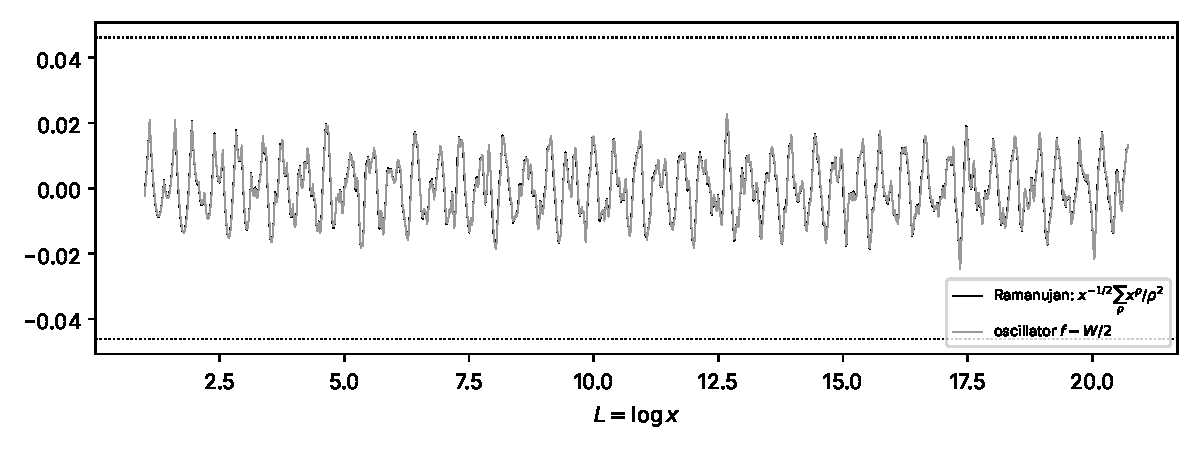
\includegraphics[width=\textwidth]{fig/v3/cl_ramanujan.pdf}
\caption{Ramanujan's normalised sum $x^{-1/2}\sum_\rho x^\rho/\rho^2$ from the primes to $10^9$ (black), the oscillator shifted by half its band (grey), and Ramanujan's band $\pm(2+\gamma_E-\log4\pi)$ (dotted).}
\label{cl:fig:ram}
\end{figure}

The constant $\log4\pi-\gamma_E$ also appears in the result for which the 1915 paper is known. Assuming RH, Ramanujan showed for his generalised superior highly composite numbers, the colossally abundant numbers of Alaoglu and Erd\H{o}s, that $\limsup(\sigma_{-1}(n)-e^{\gamma_E}\log\log n)\sqrt{\log n}\le-e^{\gamma_E}(2\sqrt2-4-\gamma_E+\log4\pi)=-1.3932$. Robin proved in 1984 \cite{Robin84} that RH is equivalent to $\sigma(n)<e^{\gamma_E}n\log\log n$ for all $n>5040$, and that if RH fails a counterexample can be found among the colossally abundant numbers. In Ramanujan's result the constant enters through $\sum_\rho1/|\rho|^2=2+\gamma_E-\log4\pi$, which is half the width of Ramanujan's band. See Nicolas and Sondow \cite{Nicolas12} for the history.

\section{Hardy and Littlewood, 1916: which zeros a criterion can see}\label{cl:sec:hl}

In 1916 Riesz proved \cite{Riesz16} that RH is equivalent to $\sum_n\mu(n)n^{-2}e^{-x/n^2}=O(x^{-3/4+\varepsilon})$; see Section~\ref{ch:riesz} for this criterion on the Thorin path. Hardy and Littlewood, in their long paper in Acta Mathematica 41 \cite{HL16}, gave the companion criterion
\[
P_1(x)=\sum_{n\ge1}\frac{\mu(n)}ne^{-x/n^2}=O\bigl(x^{-1/4+\varepsilon}\bigr),
\]
in the course of correcting an identity of Ramanujan from his second notebook, which as Ramanujan wrote it is false. They expressed $P_1$ as a sum over the zeros. The Mellin transform of $e^{-x/n^2}$ gives $P_1(x)=\frac1{2\pi i}\int\Gamma(s)x^{-s}\zeta(1-2s)^{-1}\,\mathrm{d}s$ on a line $-1<\operatorname{Re}s<0$, the pole of $\Gamma$ at $s=0$ having residue $1/\zeta(1)=0$, which is $\sum\mu(n)/n=0$. The residues at $s=(1-\rho)/2$ give
\[
x^{1/4}P_1(x)=\sum_\rho\frac{\Gamma(\frac{1-\rho}2)}{2\zeta'(\rho)}x^{i\gamma/2}+(\text{terms from the trivial zeros})
\]
under RH and the simplicity of the zeros, with brackets in the sum over zeros. The same factors appear in Remark~\ref{dl:rem:Zid} and the passage after it, in the chapter on Ramanujan's $\Delta$.

\begin{computation}\label{cl:comp:riesz}
$P_1(x)$ for $10\le x\le10^{10}$ (computed), with the M\"obius function to $3\times10^7$ and the tail of the series summed exactly through $1/\zeta(3)$, $1/\zeta(5)$ and $1/\zeta(7)$. For $x\ge10^4$, $|x^{1/4}P_1(x)|\le2\times10^{-4}$ (the maximum over $36$ sample points is $1.6\times10^{-4}$). The sum over the first $40$ zeros with the trivial terms reproduces $x^{1/4}P_1(x)$ to three or four digits at $x=10^6$ and $10^8$, where the values are $-2.964\times10^{-5}$ and $-1.216\times10^{-5}$ both directly and from the zeros. At $x=10^{10}$ the direct value is $1.920\times10^{-5}$ and the zero sum is $1.888\times10^{-5}$: the $1.7$ per cent gap is unexplained (the direct value is stable under changing the M\"obius range from $10^7$ to $3\times10^7$), and we do not claim agreement there. The amplitudes $|\Gamma(\frac{1-\rho}2)/2\zeta'(\rho)|$ of the first four zeros are $1.5\times10^{-5}$, $4.1\times10^{-8}$, $1.4\times10^{-9}$ and $2.0\times10^{-11}$.
\end{computation}

The Gamma factor decays like $e^{-\pi|\gamma|/4}$, so the Riesz and Hardy and Littlewood criteria see the first zero and, faintly, the second, and nothing else. An off line zero $\beta+i\gamma$ at height $1000$ would contribute to $x^{1/4}P_1(x)$ a term of size $e^{-785}x^{(\beta-1/2)/2}$, which no computation of $P_1$ will ever detect. The oscillator weights the zero at height $\gamma$ by $\gamma^{-2}$, and von Mangoldt's formula by $\gamma^{-1}$. This is the practical content of the choice of kernel: smoothing with $e^{-x/n^2}$ makes the series converge fast and makes the criterion blind, while smoothing by integration in $\log x$, a Riesz mean of order one in the logarithm, keeps every zero in view at the cost of only a power of $\gamma$.

Hardy and Littlewood's paper also treats $\psi(x)-x$ at the scale of $\sqrt x$, and Littlewood's theorem of 1914 \cite{Littlewood14}, that $\psi(x)-x$ is larger than $c\sqrt x\log\log\log x$ with both signs for arbitrarily large $x$, is the input to Section~\ref{bo:sec:oscdetail}, where it shows that the oscillator, bounded under RH, has unbounded speed.

\section{Hardy, Littlewood and P\'olya, 1934, and Montgomery and Vaughan}\label{cl:sec:hlp}

\emph{Inequalities} \cite{HLP34} was written as a systematic treatment of the standard inequalities of analysis, among them Hilbert's inequality, to which its Chapter IX is devoted. Its descendant, the inequality of Montgomery and Vaughan \cite{MV74}, states in the quadratic form that for real $\lambda_r$ with $\delta_r=\min_{s\ne r}|\lambda_r-\lambda_s|>0$,
\[
\Bigl|\sum_{r\ne s}\frac{a_r\bar a_s}{\lambda_r-\lambda_s}\Bigr|\le\frac{3\pi}2\sum_r\frac{|a_r|^2}{\delta_r}.
\]
The bilinear form follows, since $i/(\lambda_r-\lambda_s)$ is hermitian. It gives the finite range form of the mean values of Proposition~\ref{bo:prop:averages}, which were stated only as limits.

\begin{proposition}[Finite window]\label{cl:prop:window}
Let $S(L)=\sum_rc_re^{i\lambda_rL}$ be a finite sum with distinct real frequencies. For every $L_0$ and $X>0$,
\[
\Bigl|\frac1X\int_{L_0}^{L_0+X}|S(L)|^2\,\mathrm{d}L-\sum_r|c_r|^2\Bigr|\le\frac{3\pi}X\sum_r\frac{|c_r|^2}{\delta_r}.
\]
\end{proposition}

\begin{proof}
Expanding, the integral is $X\sum|c_r|^2$ plus $\sum_{r\ne s}c_r\bar c_s\bigl(e^{i(\lambda_r-\lambda_s)(L_0+X)}-e^{i(\lambda_r-\lambda_s)L_0}\bigr)/(i(\lambda_r-\lambda_s))$. Each of the two parts is a form of Montgomery and Vaughan's type with $a_r=c_re^{i\lambda_rL}$ at $L=L_0+X$ and at $L=L_0$, so each is at most $\frac{3\pi}2\sum|c_r|^2/\delta_r$ in modulus.
\end{proof}

\begin{computation}\label{cl:comp:window}
Under RH, $f-\langle f\rangle=-\sum_{\gamma>0}2\gamma^{-2}\cos\gamma L$. Applied to the zeros below $7000$, with their actual gaps, and with the higher zeros bounded through $\sum_{\gamma>7000}2\gamma^{-2}\le3.7\times10^{-4}$ and Cauchy's inequality, the proposition gives for the window $4\le L\le20.72$ of Computation~\ref{bo:comp:oscdeep}: the mean square of $f$ about its window mean lies in $[6.0\times10^{-5},9.0\times10^{-5}]$ (computed). The value from the primes to $10^9$ is $7.41\times10^{-5}$ (computed). The term from Hilbert's inequality is $8.4\times10^{-6}$, of which $4.1\times10^{-6}$, about half, comes from the first zero, whose nearest gap is $\gamma_2-\gamma_1=6.89$.
\end{computation}

So the computed mean square is consistent with RH with an explicit error, over a window of finite length, which the limit statement of Proposition~\ref{bo:prop:averages} could not give. The same estimate applied to $f'$ would give a finite window form of the simplicity test, the first open problem of Section~\ref{bo:sec:oscq}, except that the series for $f'$ converges only in mean square, so the higher zeros can no longer be bounded by absolute convergence and need a bound on their gaps on average. That is the remaining step.

P\'olya's own contribution to the subject is older and appears in Volumes I and II: his 1926 study \cite{Polya} of the integral representation of $\xi$ and of Fourier transforms with only real zeros, which is the starting point of the Riemann density and the de Bruijn Newman family.

\section{The $2\sin^2$ kernel as the common thread}\label{cl:sec:sin2}

The identity $1-\cos\theta=2\sin^2(\theta/2)$ turns the oscillator into a sum of nonnegative terms, $f(L)=\sum_{\gamma>0}4\sin^2(\gamma L/2)/\gamma^2$, so that the band is $[0,W]$ and the lower wall is a positivity statement rather than a two sided bound. This part of the chapter is already in Volume II. The oscillator is $f=D/2$ with $D$ of Proposition~\ref{yo:prop:tent}(b), the Fej\'er and triangle Fourier pair is Proposition~\ref{yo:prop:tent}(a), the explicit formula for the Fej\'er weights is half of Proposition~\ref{yo:prop:tent}(c) and (d), and the criterion is Theorem~\ref{yo:thm:D}. We do not reprint them. Positivity of this type, in the language of screw functions, is the subject of Suzuki \cite{Suzuki22}, and a positivity property of $\xi$ equivalent to RH is due to Lagarias \cite{Lagarias}; Volume II relates the screw function approach to Theorem~\ref{yo:thm:D}. % UNCHECKED: the term by term match of normalisations with Suzuki22 and Lagarias was not checked here

Three remarks are specific to this chapter.

Ramanujan's sum is not of this form. His terms $2\operatorname{Re}\,e^{i\gamma L}/(\frac12+i\gamma)^2$ have no sign, and his sum equals $f-\frac W2$ plus a series of terms of size $\gamma^{-3}$. Both are criteria by Landau's theorem (Theorem~\ref{cl:thm:band}), but only the $2\sin^2$ form gives positivity term by term, which is what the later results of Chapter~\ref{bo:ch:bondesson} use.

The kernel $e^{-x/n^2}$ of Riesz and of Hardy and Littlewood has no such form. It produces Gamma weights at the zeros, the weights decay like $e^{-\pi\gamma/4}$, and there is no positivity, only an $O$ bound.

The cancellation ledger of Theorem~\ref{bo:thm:ledger} contains a $2\sin^2$ transform over the primes in the height variable $t$, while the oscillator is a $2\sin^2$ transform over the zeros in the variable $L=\log x$. The kernel is the same function $2\sin^2(ab/2)$ of a product of two variables with the pairs exchanged, $(t,\log y)$ in the ledger and $(\gamma,L)$ in the oscillator. We read the two as the two sides of one explicit formula. This is a heuristic remark, not a theorem.

The kernel gives positivity term by term only when every $\gamma$ is real, which is RH. At a zero off the line, $\gamma=\gamma_0-i\delta$, the kernel becomes a mixture of $\cosh$ and $\cos$ and can be negative; Lemma~\ref{bo:lem:offline} measures how far, at most $(\cosh(\delta h)-1)(1+\kappa)/|\rho-\frac12|^2$, where $h$ plays the role of $L$ and $\kappa=4\delta^2/(\gamma_0^2-\delta^2)$. So the kernel does not add a proof. It identifies the positivity that every criterion in this chapter is about.

\section{What the classics add}\label{cl:sec:add}

The oscillator has ancestors. Von Mangoldt's formula, weighted by $x^{-1/2}$ and differentiated, is its second derivative. Ramanujan's bound of 1915 is a symmetric band of nearly the same width, $2\sum_\rho|\rho|^{-2}=0.09238$ against $W=0.09242$, centred differently; with Landau's theorem a bound of this kind is a criterion. What the readings add is a sharper sense of why this particular object is useful. Its weights $\gamma^{-2}$ keep every zero visible, where the exponential kernels of Riesz and of Hardy and Littlewood keep only the first. Its centre at $\rho=\frac12$ starts the band at zero, where Ramanujan's centre at $\rho=0$ leaves it symmetric; the oscillator is Ramanujan's sum written in $2\sin^2$ form, up to a series of size $10^{-3}$. And the inequality of Montgomery and Vaughan \cite{MV74} turns its limiting statements into statements about finite ranges of $x$, which is where computation lives.

None of this brings RH closer. It does say that RH in its oscillator form (Theorem~\ref{bo:thm:osc}), a two sided bound on $\sum_{n\le x}\Lambda(n)n^{-1/2}\log(x/n)$ after subtracting an explicit function, is close to what Ramanujan's 1915 bound already expressed under RH, and that what has been missing for a century is not the formulation but a way to control the prime sum over every range at once.
